%%%% utfprpgtex-slides.tex, 2019/02/21
%%%% Copyright (C) 2015-2019 Luiz E. M. Lima (luizeduardomlima@gmail.com)
%%
%% Este arquivo pode ser distribuído e/ou modificado sob as condições da
%% Licença Pública do Projeto LaTeX, tanto a versão 1.3 desta licença ou (à sua
%% opção) qualquer versão posterior.
%% A versão mais recente desta licença está disponível em
%%   http://www.latex-project.org/lppl.txt
%% e a versão 1.3 ou posterior faz parte de todas as distribuições de LaTeX
%% versão 2005/12/01 ou posterior.
%%
%% Este arquivo tem o estado de manutenção da LPPL `mantida'.
%%
%% O mantenedor atual deste arquivo é Luiz E. M. Lima.
%%
%% Este projeto consiste dos arquivos utfprpgtex-slides.sty e
%% utfprpgtex-slides.tex.
%%
%% utfprpgtex-slides.tex é o arquivo principal do modelo LaTeX (não oficial)
%% para produção de apresentação de slides da Universidade Tecnológica Federal
%% do Paraná (UTFPR). Foi desenvolvido baseado no modelo de apresentação de
%% slides do abnTeX2, disponível em <http://www.abntex.net.br/>, criado por
%% Fábio Rodrigues Silva usando a classe beamer, disponível em
%% <http://ctan.org/pkg/beamer/>.

%% Classe e opções de documento
%%%% Modo apresentação --- Descomente o comando \documentclass[]{beamer}
\documentclass[%% Opções
  xcolor=table,%%
  10pt,%% Tamanho de fonte: 10pt, 11pt, 12pt, etc.
  aspectratio = 169,%% Razão de aspecto: 1610 (16:10), 169 (16:9), 149 (14:9), 54 (5:4), 43 (4:3 - padrão) e 32 (3:2)
  compress,%% Tenta reduzir o tamanho das barras de navegação (comente para desabilitar)
  t,%% Alinhamento vertical dos quadros: b (fundo), c (centro) e t (topo)
  % handout,%% Cria uma versão que usa as especificações de sobreposição do folheto (comente para desabilitar)
]{beamer}%% Classe beamer
%%%% Modo artigo --- Descomente os comandos \documentclass[]{article} e \usepackage{beamerarticle}
% \documentclass[a4paper, twocolumn]{article}%% Classe artigo
% \usepackage{beamerarticle}%% Utiliza o modo artigo da classe beamer

%% Passagem de opções para pacotes
\PassOptionsToPackage{english, main = brazilian}{babel}%% Suporte multilíngue

%% Pacotes utilizados
\usepackage{utfprpgtex-slides}%% Estilos do modelo
\usepackage{multirow}

%% Arquivo de referências
\addbibresource{utfprpgtex-slides.bib}
\addtobeamertemplate{footline}{\hypersetup{allcolors=.}}{}

%% Arquivos de logomarcas (presentes no diretório ``Logos'') --- Deixe o campo {} vazio ou comente para remover
\logoprog{logo-ppgbioinfo}%% Logomarca do programa ou do curso
\logocampus{logo-utfpr}%% Logomarca do câmpus

\title[Classificação de TEs por CNNs]{%% Título da apresentação: [curto] e {longo}
  \texorpdfstring{\mode<article>{\bfseries}}{}%% Modo artigo --- Negrito
  Classificação de Elementos Transponíveis por Redes Neurais Convolucionais
}

\subject{Defesa da Proposta de Dissertação de Mestrado}%% Assunto da apresentação, e.g.: {Nome do Evento}
\author[M. H. P. da Cruz]{%% Autor(a): [curto] e {longo}
  Murilo Horácio Pereira da Cruz%
  \authormail{murilocruz@alunos.utfpr.edu.br}%
  \advisor{Orientador: Prof. Dr. Pedro Henrique Bugatti}%
  \advisor{Co-Orientador: Prof. Dr. Alexandre Rossi Paschoal}%
}

\institute[UTFPR-CP/DACOM/PPGBIOINFO]{%% Instituição: [curto] e {longo}
  \utfprname, Câmpus Cornélio Procópio (UTFPR-CP)%
  \par Departamento de Computação (DACOM)%
  \par Programa de Pós-Graduação em Bioinformática (PPGBIOINFO)%
}
\titlegraphic{%% Logomarcas da instituição
  \vspace*{-\baselineskip}%
  \institutelogos%
}
\campus{CP}{Câmpus Cornélio Procópio}%% Câmpus: {sigla} e {nome} --- Modo artigo
%\departamento[logo-da]{<DEPTO>}{%% Depto., Coord., Prog. ou Curso: [logo], {sigla} e {nome} --- Modo artigo
%  Departamento Acadêmico de <Nome do Depto.>%
%}
\date[\today]{}%% Data: [curto] e {longo}

%% Início do documento
\begin{document}

\mode<presentation>{%% Modo apresentação --- Páginas de título e de sumário
  \frame{\titlepage}%
  \begin{frame}{Sumário}{~}%
    \frametitle{Sumário}
    \tableofcontents%
  \end{frame}%
}

\mode<article>{%% Modo artigo --- Página de título
  \maketitle%
  \thispagestyle{firstpagestyle}%
}

% ----------------------------- INTRODUÇÃO -----------------------------%
\section{Introdução}\label{sec:intro}

\begin{frame}{\sectiontitle{sec:intro}}{Elementos Transponíveis}
    \mode<presentation>{\vfill}
    \begin{columns}
        \begin{column}{0.5\textwidth}
            \begin{itemize}
                \item Barbara McClintock
                \item Alteração da pigmentação em grãos de milho
                \item Genoma Dinâmico
                \item Sequências que produzem cópias ao longo do genoma
                \item Sequências que se locomovem ao longo do genoma
                \item Consequências
                \item Presentes em grandes quantidades
            \end{itemize}       
        \end{column}
        \begin{column}{0.5\textwidth}  %%<--- here
            \begin{center}
                \begin{figure}
                    \centering
                    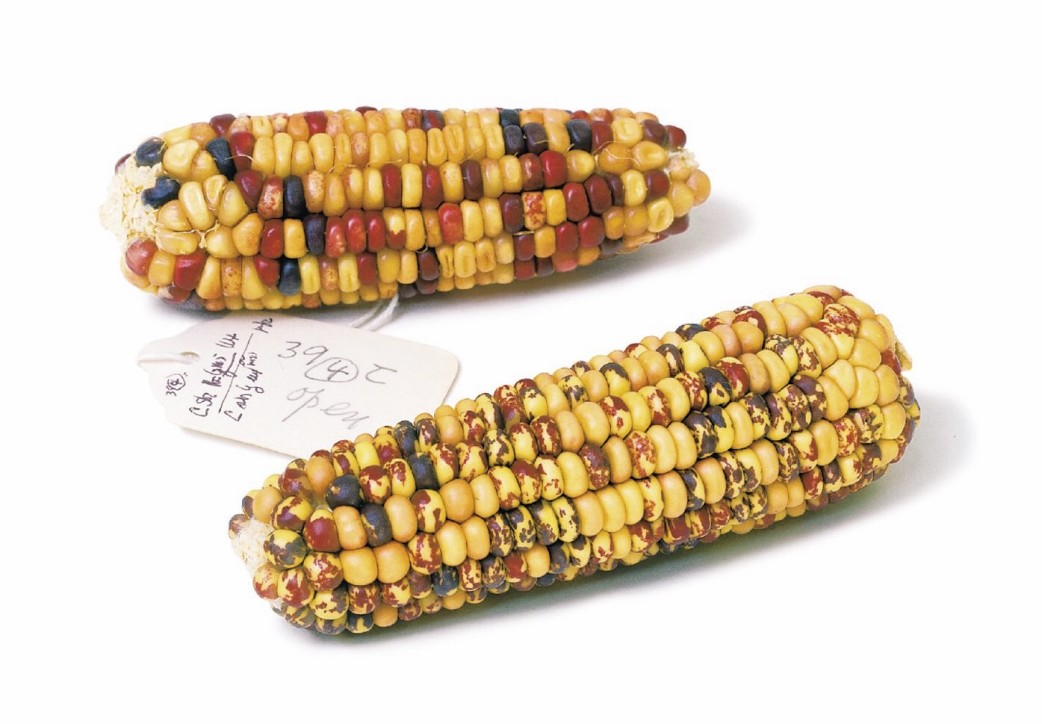
\includegraphics[width = 0.7\textwidth]{./Figuras/te-maize.jpg}
                    \caption{Instabilidade no fenótipo do milho causada pela ação de TEs}
                    \scriptsize Fonte: www.nobelprize.org %https://www.nobelprize.org/womenwhochangedscience/stories/barbara-mcclintock
                    \label{fig:maize-phenotype-instability}
                \end{figure}
             \end{center}
        \end{column}
    \end{columns}
\end{frame}

\begin{frame}{\sectiontitle{sec:intro}}{Mecanismos de Transposição}
    \mode<presentation>{\vfill}
    \begin{figure}
        \centering
        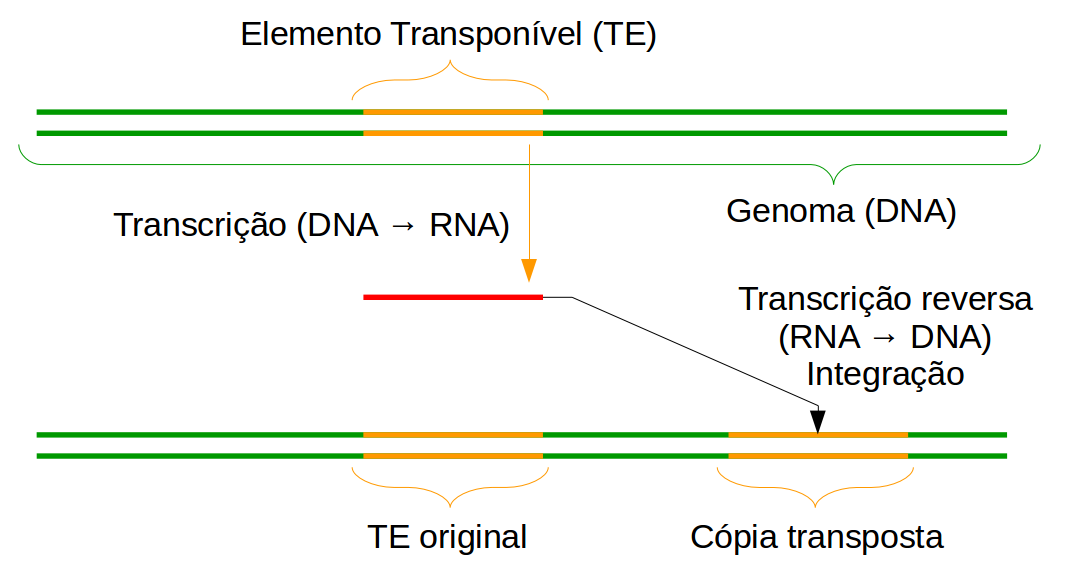
\includegraphics[width=0.7\textwidth]{./Figuras/retrotransposons.png}
        \caption{Mecanismo de transposição dos retrotransposons}
        \label{fig:transposition-1}
    \end{figure}
\end{frame}

\begin{frame}{\sectiontitle{sec:intro}}{Mecanismos de Transposição}
    \mode<presentation>{\vfill}
    \begin{figure}
        \centering
        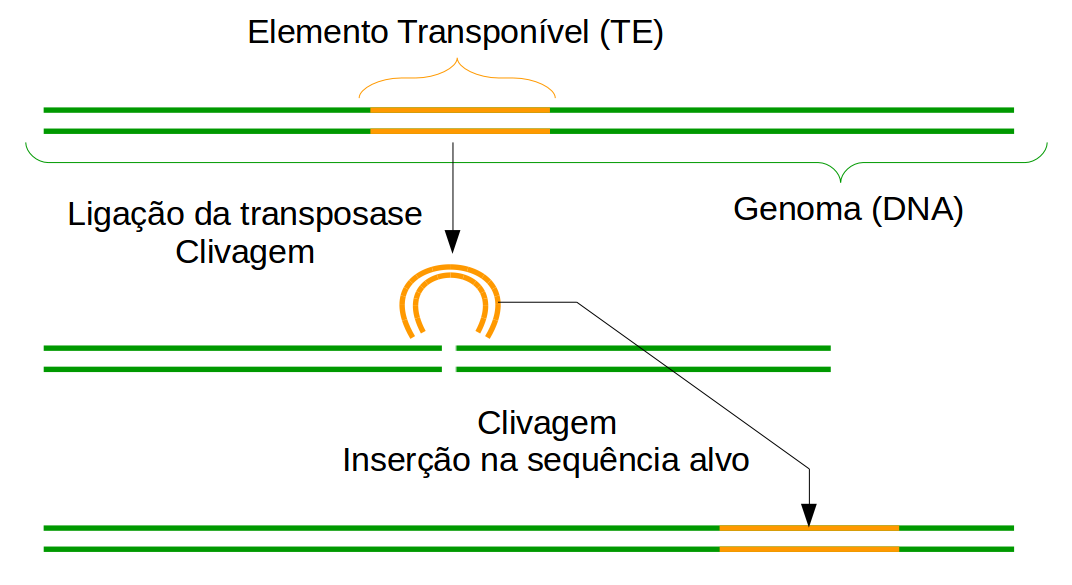
\includegraphics[width=0.7\textwidth]{./Figuras/transposons.png}
        \caption{Mecanismo de transposição dos elementos da Classe II}
        \label{fig:transposition-2}
    \end{figure}
\end{frame}

\begin{frame}{\sectiontitle{sec:intro}}{Classificação de Elementos Transponíveis}
    \mode<presentation>{\vfill}
    \begin{figure}
        \centering
        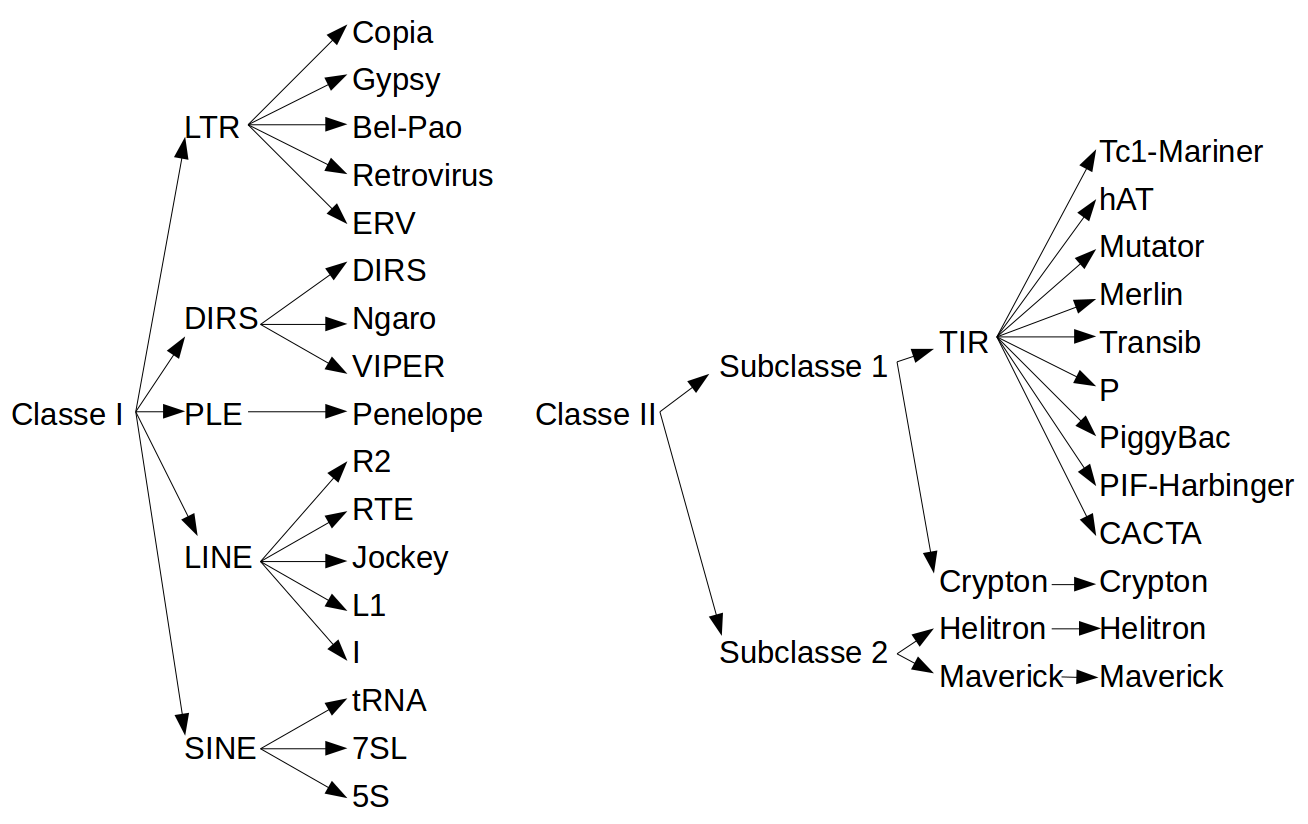
\includegraphics[width=0.6\textwidth]{./Figuras/te-classes.png}
        \caption{Classificação de TEs segundo \cite{Wicker2007}}
        \label{fig:classes}
    \end{figure}
\end{frame}

\begin{frame}{\sectiontitle{sec:intro}}{Classificação de Elementos Transponíveis}
    \mode<presentation>{\vfill}
    \begin{figure}
        \centering
        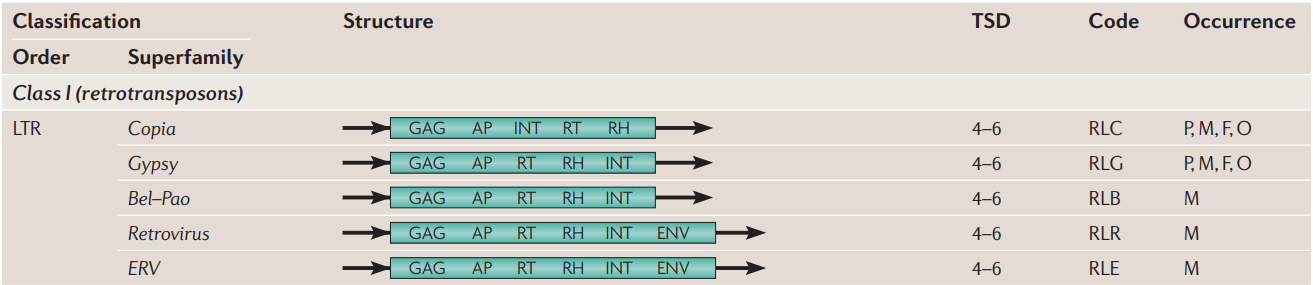
\includegraphics[width=0.8\textwidth]{./Figuras/LTR-structures.png}
        \caption{Estruturas dos TEs segundo \cite{Wicker2007}}
        \scriptsize Fonte: \cite{Wicker2007}
        \label{fig:ltr-structures}
    \end{figure}
    \begin{itemize}
        \item Mesmo mecanismo de transposição
        \item Elementos com mesma estrutura podem possuir origens diferentes
        \item Mesmo complexo proteico pode produzir produtos diferentes
    \end{itemize}
\end{frame}

\begin{frame}{\sectiontitle{sec:intro}}{Redes Neurais Convolucionais}
    \mode<presentation>{\vfill}
    \begin{block}{Redes Neurais Convolucionais (CNNs)}
        \begin{itemize}
            \item \textit{Representation Learning}
            \item \textit{Deep Learning}
            \item Extração de características
            \item Aprender filtros 
            \item Conexões esparsas
            \item Invariância espacial
            \item Redução da complexidade (dimensão)
        \end{itemize}
    \end{block}
\end{frame}

\begin{frame}{\sectiontitle{sec:intro}}{Operação de Convolução}
    \mode<presentation>{\vfill}
    \begin{center}
        \begin{figure}
            \centering
            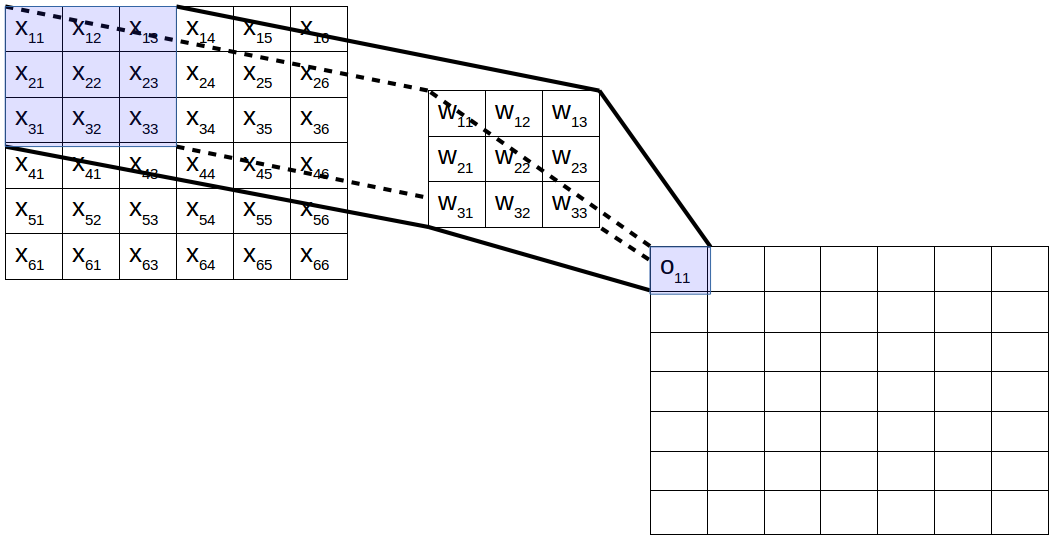
\includegraphics[width=0.6\textwidth]{./Figuras/conv-op-1.png}
            \caption{Operação de convolução}
        \end{figure}
        $o = \phi(\sum_{i,j=1}^{n} x_{ij}w_{ij} + b)$
    \end{center}
\end{frame}

\begin{frame}{\sectiontitle{sec:intro}}{Operação de Convolução}
    \mode<presentation>{\vfill}
    \begin{center}
        \begin{figure}
            \centering
            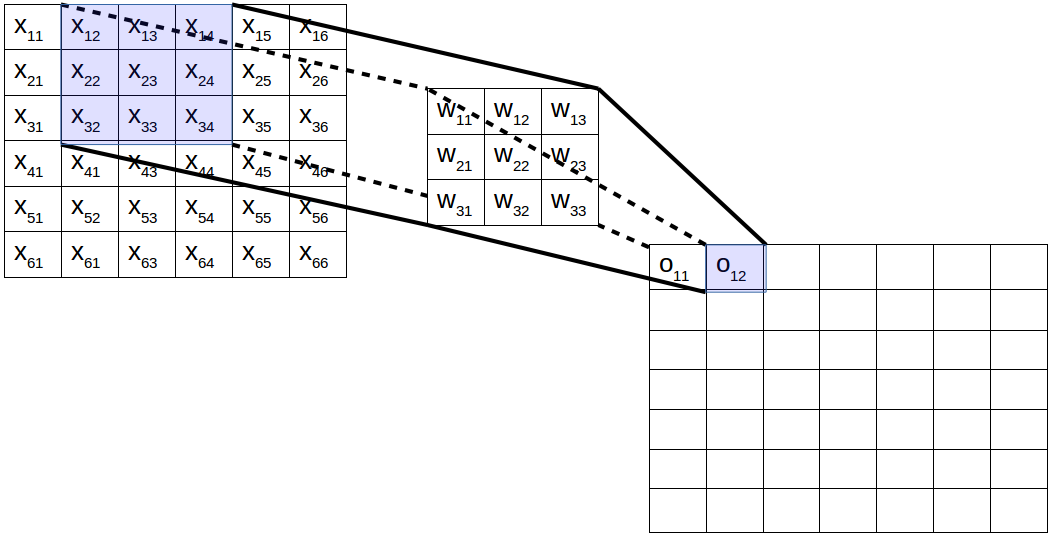
\includegraphics[width=0.6\textwidth]{./Figuras/conv-op-2.png}
            \caption{Operação de convolução}
        \end{figure}
        $o = \phi(\sum_{i,j=1}^{n} x_{ij}w_{ij} + b)$
    \end{center}
\end{frame}

\begin{frame}{\sectiontitle{sec:intro}}{Operação de Convolução}
    \mode<presentation>{\vfill}
    \begin{center}
        \begin{figure}
            \centering
            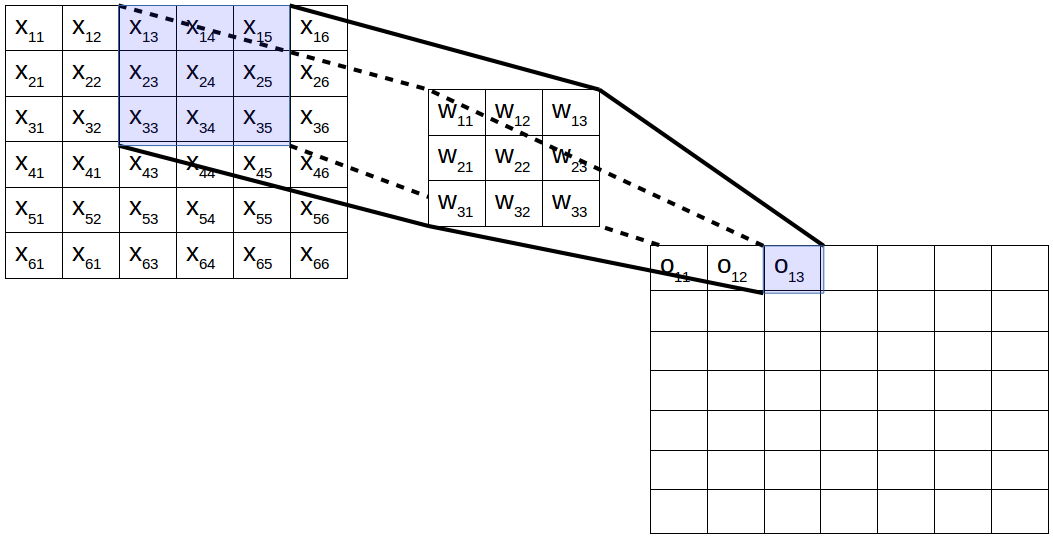
\includegraphics[width=0.6\textwidth]{./Figuras/conv-op-3.png}
            \caption{Operação de convolução}
        \end{figure}
        $o = \phi(\sum_{i,j=1}^{n} x_{ij}w_{ij} + b)$
    \end{center}
\end{frame}

\begin{frame}{\sectiontitle{sec:intro}}{Operação de Pooling}
    \mode<presentation>{\vfill}
    \begin{figure}
        \centering
        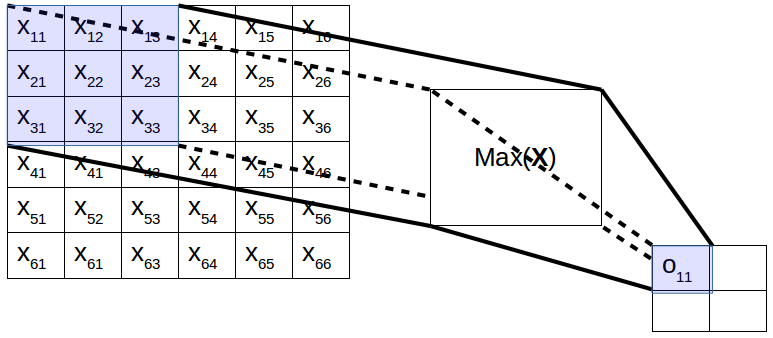
\includegraphics[width=0.6\textwidth]{./Figuras/pool-op-1.png}
        \caption{Operação de \textit{max pooling}}
    \end{figure}
\end{frame}

\begin{frame}{\sectiontitle{sec:intro}}{Operação de Pooling}
    \mode<presentation>{\vfill}
    \begin{figure}
        \centering
        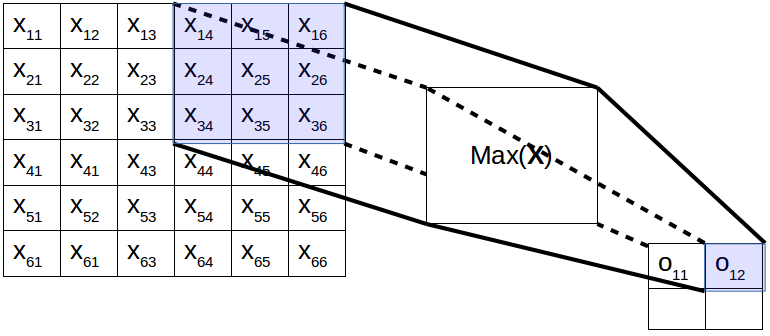
\includegraphics[width=0.6\textwidth]{./Figuras/pool-op-2.png}
        \caption{Operação de \textit{max pooling}}
    \end{figure}
\end{frame}

\begin{frame}{\sectiontitle{sec:intro}}{Operação de Pooling}
    \mode<presentation>{\vfill}
    \begin{figure}
        \centering
        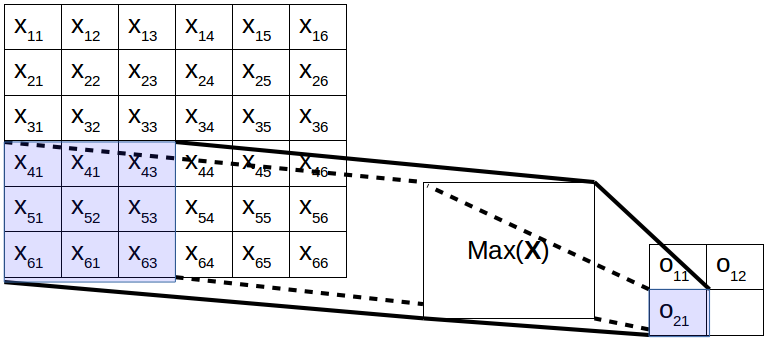
\includegraphics[width=0.6\textwidth]{./Figuras/pool-op-3.png}
        \caption{Operação de \textit{max pooling}}
    \end{figure}
\end{frame}

\begin{frame}{\sectiontitle{sec:intro}}{Arquiteturas de CNNs}
    \mode<presentation>{\vfill}
    \begin{figure}
        \centering
        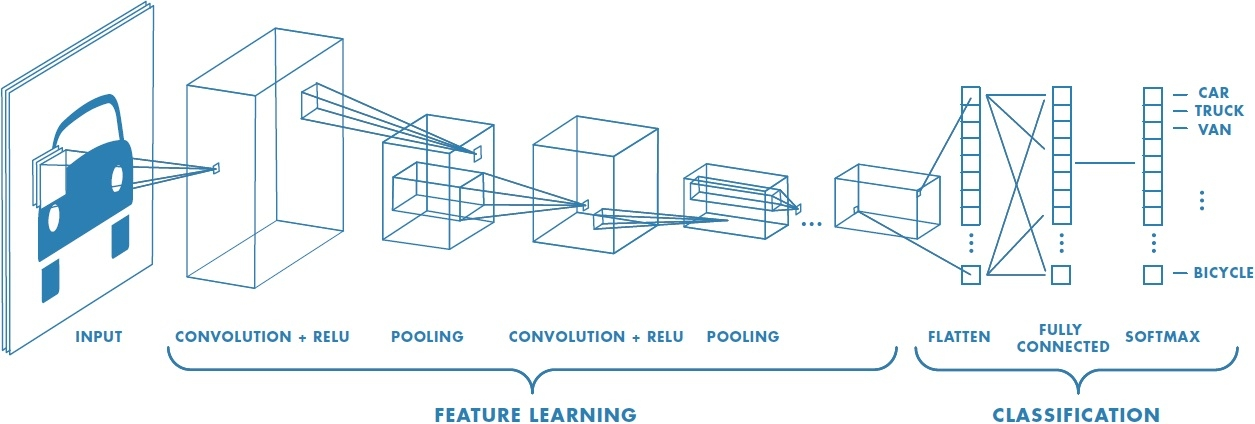
\includegraphics[width=0.8\textwidth]{./Figuras/cnn-architecture.jpg}
        \caption{Arquitetura de uma CNN}
        \scriptsize Fonte: www.mathworks.com
    \end{figure}
\end{frame}
% ----------------------- REVISÂO DA LITERATURA ------------------------%
\section{Revisão da Literatura}\label{sec:revlit}

\begin{frame}{\sectiontitle{sec:revlit}}{TEclass}
    \begin{block}{\textit{TEclass — A Tool for Automated Classification of Unknown Eukaryotic Transposable Elements}}
        \begin{itemize}
            \item Propõem classificar TEs nas classes: \textbf{DNA transposons, LTR, LINE e SINE}
            \item Utiliza \textbf{\textit{k-mers}} com $k={4,5}$ e similaridade como características
            \item Utiliza a base RepBase como base de busca por \textbf{similaridade}
            \item Modelos específicos para \textbf{faixas de comprimento}
            \item Aplica classificação binária utilizando \textbf{SVM} 
            \item Classifica sequências do RepBase de uma versão mais recente que a base para similaridade
            \item Obteve cerca de 90 a 97\% de acurácia para DNA transposons e LTR
            \item Obteve cerca de 75\% de acurácia para LINEs e SINEs
        \end{itemize}
    \end{block}
\end{frame}

\begin{frame}{\sectiontitle{sec:revlit}}{TEclass}
    \mode<presentation>{\vfill}
    \begin{figure}
        \centering
        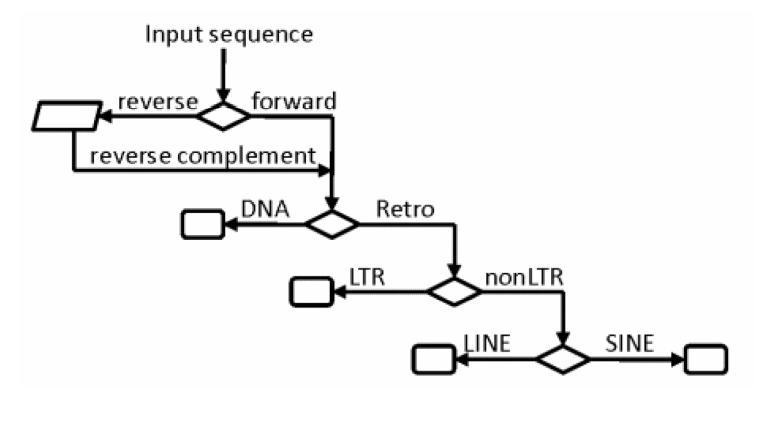
\includegraphics[width=0.6\textwidth]{./Figuras/workflow-teclass.png}
        \caption{Diagrama da operação de classificação realizada pelo método TEclass}
        \scriptsize Fonte: \cite{teclass}
    \end{figure}
\end{frame}

\begin{frame}{\sectiontitle{sec:revlit}}{PASTEC}
    \begin{block}{\textit{PASTEC: An Automatic Transposable Element Classification Tool}}
        \begin{itemize}
            \item Classifica TEs por meio de características estruturais e similaridade
            \item Utiliza HMMs para classificar TEs por meio de inferência
            \item Através das HMMs consegue obter um perfil para classificação de cada classe e ordem
            \item Perfil que tiver melhor ativação é a resposta da classificação
            \item Utiliza as características: comprimento da sequência, LTR, TIR, SSR, cauda polyA e ORFs
            \item Melhor acurácia obtida: 80.7\% (para classificação de apenas 318 sequências)
            \item Possui baixa taxa de falsa classificação
        \end{itemize}
    \end{block}
\end{frame}

\begin{frame}{\sectiontitle{sec:revlit}}{PASTEC}
    \mode<presentation>{\vfill}
    \begin{figure}
        \centering
        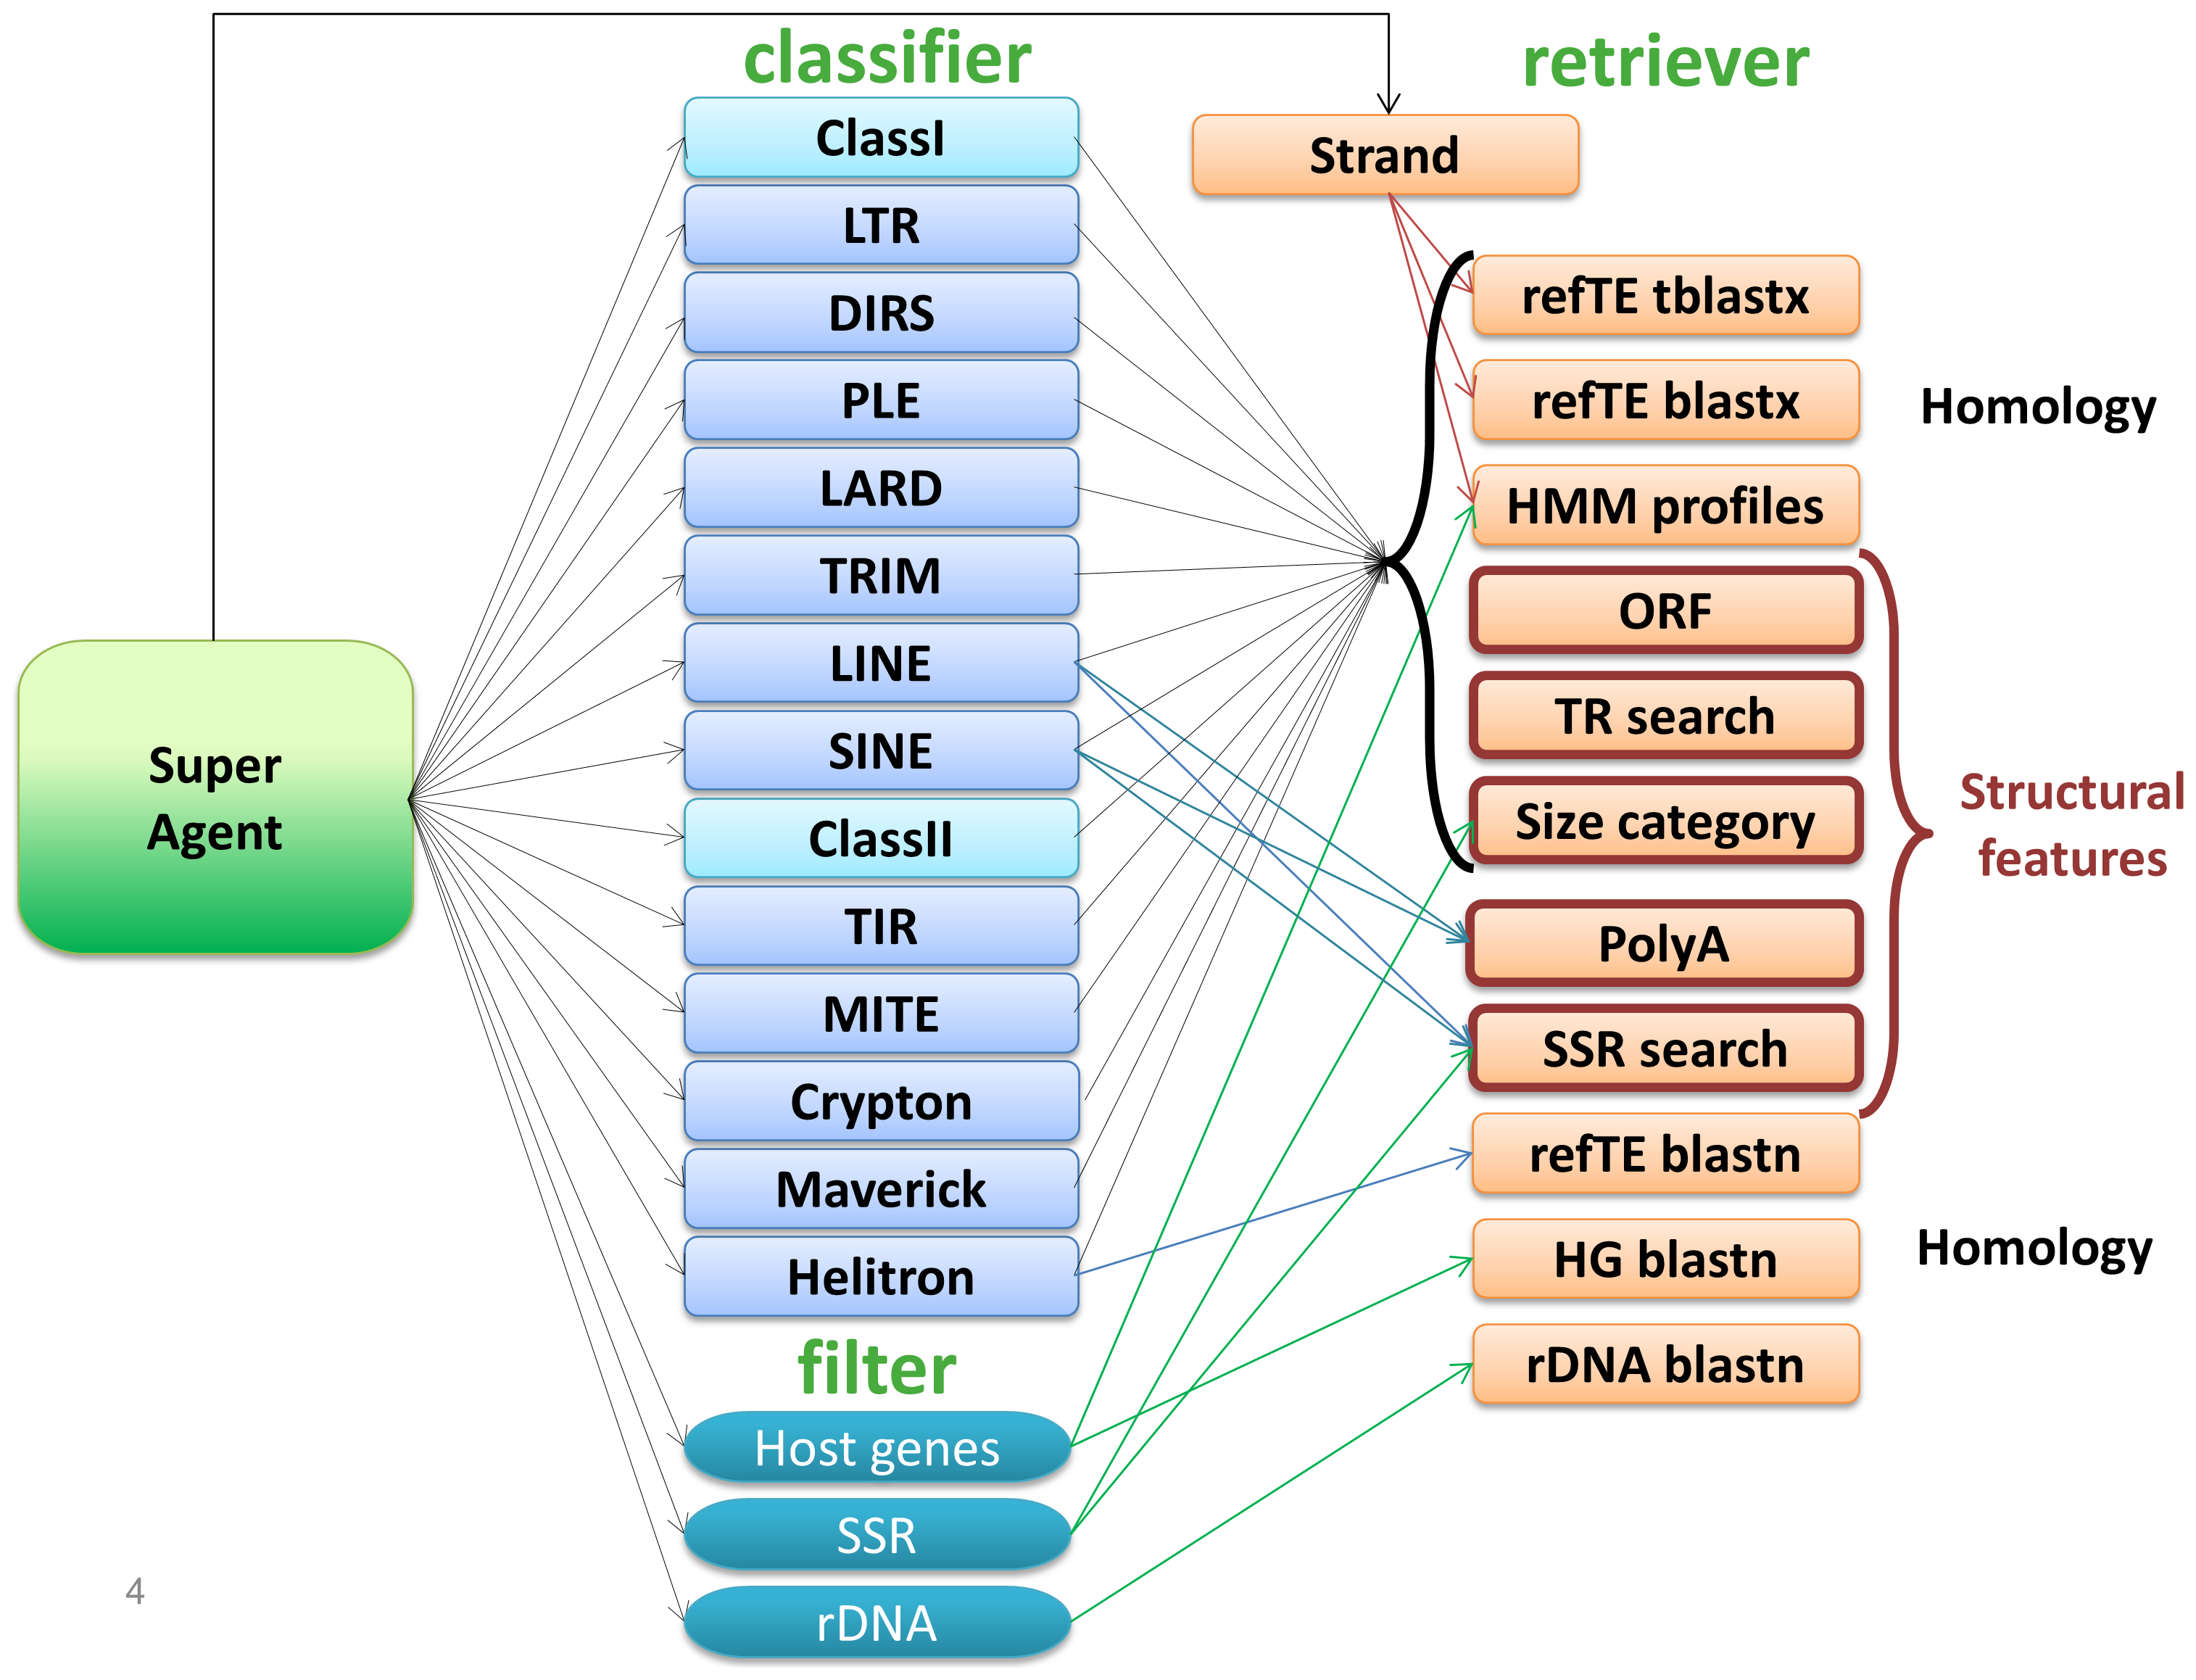
\includegraphics[width=0.5\textwidth]{./Figuras/workflow-pastec.png}
        \caption{Diagrama da operação de classificação realizada pelo método PASTEC}
        \scriptsize Fonte: \cite{pastec}
    \end{figure}
\end{frame}

\begin{frame}{\sectiontitle{sec:revlit}}{REPCLASS}
    \begin{block}{\textit{PASTEC: An Automatic Transposable Element Classification Tool}}
        \begin{itemize}
            \item Classificação genérica (qualquer classe)
            \item Classificação baseada no resultado de três módulos (similaridade, estrutural e TSD)
            \item Busca por similaridade é realizada com base nas sequências do RepBase
            \item Utiliza os elementos estruturais LTR, TIR, tRNA, cauda polyA, SSR, TSD entre outros \textit{motifs}
            \item Realiza busca por TSD na sequência candidata e a classifica com base no TSD se houver
            \item O resultado da classificação depende dos 3 módulos
        \end{itemize}
    \end{block}
\end{frame}

\begin{frame}{\sectiontitle{sec:revlit}}{REPCLASS}
    \mode<presentation>{\vfill}
    \begin{figure}
        \centering
        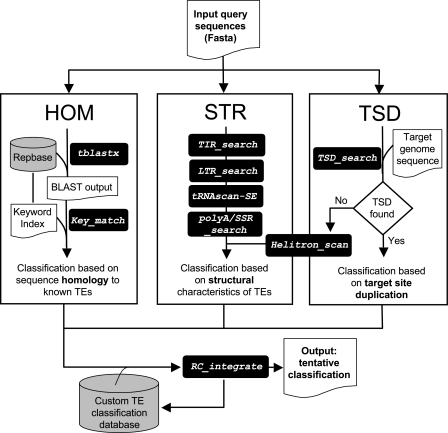
\includegraphics[width=0.4\textwidth]{./Figuras/workflow-repclass.jpg}
        \caption{Diagrama da operação de classificação realizada pelo método REPCLASS}
        \scriptsize Fonte: \cite{repclass}
    \end{figure}
\end{frame}

% ----------------------- MATERIAIS E MÉTODOS ------------------------%
\section{Materiais e Métodos}\label{sec:matmet}

\begin{frame}{\sectiontitle{sec:matmet}}{Método Proposto}
    \mode<presentation>{\vfill}
    \begin{block}{Método Proposto}
        \begin{itemize}
            \item Utilizar CNNs para classificar TEs a nível de superfamília
            \item Não depender de características manualmente definidas
            \item Aprender a melhor representação para as sequências (extração de características)
            \item Classificar as sequências utilizando \textit{deep learning}
            \item Não depender de busca por similaridade
            \item Utilização de GPUs acelerando o processo de classificação
        \end{itemize}
    \end{block}
\end{frame}

\begin{frame}{\sectiontitle{sec:matmet}}{Pré-processamento}
    \mode<presentation>{\vfill}
    \begin{block}{Pré-processamento}
        \begin{itemize}
            \item Remover qualquer sequência repetida dos conjuntos de treinamento e teste
            \item Substituir qualquer nucleotídeo encontrado que não esteja no conjunto ${A,C,G,T,N}$ como $N$
            \item Verificar qual o maior comprimento dentre as sequências das bases
            \item Estender as demais sequências aplicando \textit{padding} para normalizar os comprimentos com base no maior comprimento
            \item Um símbolo diferente é utilizado para o \textit{padding}
            \item Aplicar a codificação \textit{one-hot encoding}
        \end{itemize}
    \end{block}
\end{frame}

\begin{frame}{\sectiontitle{sec:matmet}}{Pré-processamento}
    \mode<presentation>{\vfill}
    \begin{figure}
        \centering
        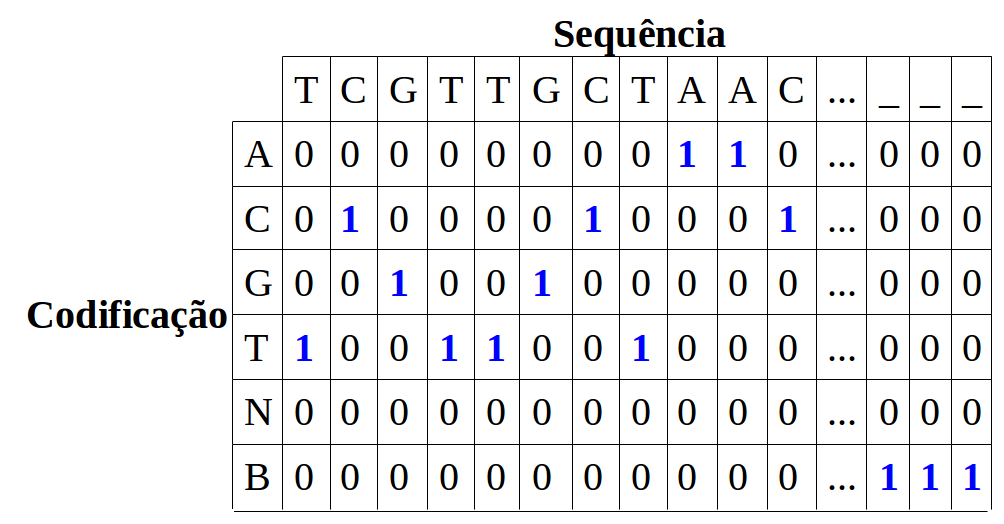
\includegraphics[width=0.6\textwidth]{./Figuras/one-hot-pt.png}
        \caption{Codificação \textit{One-Hot}}
        \label{fig:one-hot}
    \end{figure}
\end{frame}

\begin{frame}{\sectiontitle{sec:matmet}}{\textit{Pipeline}}
    \mode<presentation>{\vfill}
    \begin{figure}
        \centering
        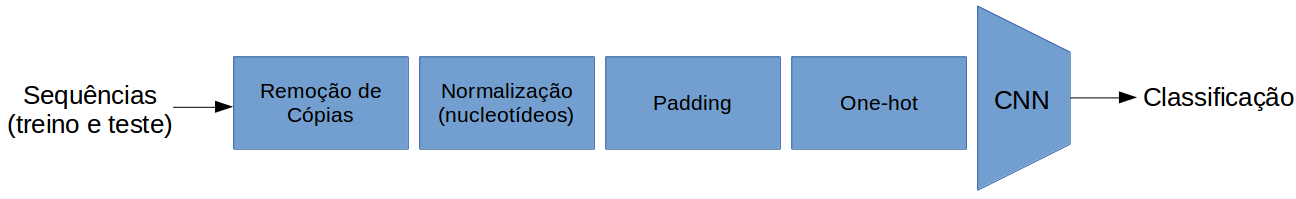
\includegraphics[width=0.9\textwidth]{./Figuras/pipeline.png}
        \caption{\textit{Pipeline} do método proposto}
        \label{fig:pipeline}
    \end{figure}
\end{frame}

% ---------------------- EXPERIMENTOS E RESULTADOS -----------------------%
\section{Experimentos e Resultados}\label{sec:expres}

\begin{frame}{\sectiontitle{sec:expres}}{Arquitetura da CNN}
    \mode<presentation>{\vfill}
    \begin{figure}
        \centering
        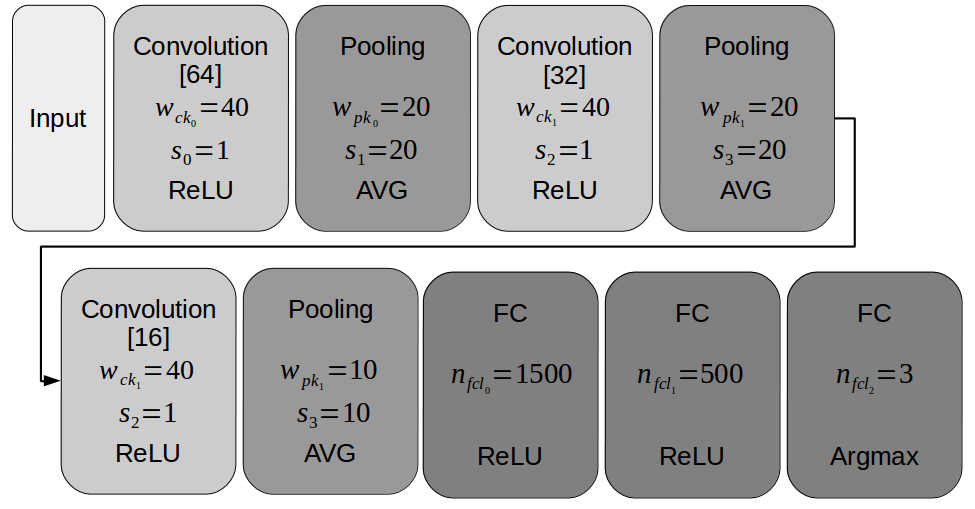
\includegraphics[width=0.6\textwidth]{./Figuras/arq-4.png}
        \caption{Arquitetura da CNN para o método proposto}
        \label{fig:arc}
    \end{figure}
\end{frame}

\begin{frame}{\sectiontitle{sec:expres}}{\textit{Datasets}}
    \begin{block}{Bases de dados}
        \begin{itemize}
            \item RepBase \cite{repbase} (mais de 100 espécies incluindo plantas, animais e fungos)
            \item DPTEdb \cite{dpte} (8 espécies de plantas)
            \item PGSB \cite{pgsb} (18 espécies de plantas)
            \item RiTE \cite{rite} (12 espécies de plantas)
            \item SPTE \cite{spte} (3 espécies de plantas)
            \item TEfam (2 espécies de mosquitos)
            \item TREP \cite{trep} (diversas espécies de plantas, bactérias e fungos)
        \end{itemize}
    \end{block}
\end{frame}

\begin{frame}{\sectiontitle{sec:expres}}{\textit{Datasets}}
    \mode<presentation>{\vfill}
    \begin{table}[]
        \centering
        \caption{Quantidade de sequências de TEs por superfamília e ordem presente em cada base de dados}
        \label{tab:datasets}
        \resizebox{0.9\textwidth}{!}{\begin{tabular}{|l|l|l|l|l|l|l|l|l|l|l|}
            \hline
            \textbf{Ordem}       & \textbf{Superfamília} & \textbf{PGSB} & \textbf{DPTE} & \textbf{TEfam} & \textbf{REPBASE} & \textbf{SPTE} & \textbf{TREP} & \textbf{RiTE} & \textbf{Total SF} & \textbf{Total Ordem}    \\ \hline
            \multirow{4}{*}{LTR} & Copia                 & 4279          & 5391          & 344            & 7030             & 2873          & 420           & 14236         & 34573             & \multirow{4}{*}{147366} \\ \cline{2-10}
                                 & Gypsy                 & 7625          & 10636         & 509            & 11185            & 8611          & 531           & 65224         & 104321            &                         \\ \cline{2-10}
                                 & Bel-Pao               & 0             & 354           & 550            & 1872             & 155           & 0             & 2             & 2933              &                         \\ \cline{2-10}
                                 & ERV                   & 0             & 655           & 0              & 4453             & 106           & 0             & 325           & 5539              &                         \\ \hline
            LINE                 & L1                    & 0             & 1386          & 114            & 1731             & 280           & 3             & 832           & 4346              & 4346                    \\ \hline
            SINE                 & SINE                  & 191           & 0             & 0              & 797              & 0             & 0             & 3240          & 4228              & 4228                    \\ \hline
            \multirow{5}{*}{TIR} & Tc1-Mariner           & 357           & 50            & 32             & 2591             & 0             & 569           & 20392         & 23991             & \multirow{5}{*}{169796} \\ \cline{2-10}
                                 & hAT                   & 81            & 113           & 42             & 3047             & 40            & 25            & 3746          & 7094              &                         \\ \cline{2-10}
                                 & Mutator               & 320           & 23            & 4              & 1382             & 8             & 165           & 106055        & 107957            &                         \\ \cline{2-10}
                                 & PIF-Harbinger         & 141           & 94            & 12             & 1131             & 11            & 155           & 18111         & 19655             &                         \\ \cline{2-10}
                                 & CACTA                 & 720           & 0             & 0              & 747              & 0             & 326           & 9306          & 11099             &                         \\ \hline
            Helitron             & Helitron              & 15            & 4652          & 5              & 980              & 3009          & 28            & 6426          & 15115             & 15115                   \\ \hline
        \end{tabular}}
    \end{table}
\end{frame}

\begin{frame}{\sectiontitle{sec:expres}}{\textit{Datasets}}
    \mode<presentation>{\vfill}
    \begin{table}
        \centering
        \caption{\textit{Dataset} 1 composto por sequências do RepBase para treino e teste}
        \label{tab:dataset1}
        \begin{tabular}{|l|l|l|l|l|}
            \hline
            \rowcolor[HTML]{C0C0C0} 
            \textbf{Ordem}              & \textbf{Superfamília}          & \textbf{Sequências}         & \textbf{Treino}            & \textbf{Teste}             \\ \hline
            {\color[HTML]{CB0000} LTR}  & {\color[HTML]{CB0000} Bel-Pao} & {\color[HTML]{CB0000} 1872} & {\color[HTML]{CB0000} 800} & {\color[HTML]{CB0000} 200} \\ \hline
            \rowcolor[HTML]{EFEFEF} 
            LTR                         & Copia                          & 7030                        & 800                        & 200                        \\ \hline
            LTR                         & ERV                            & 4453                        & 800                        & 200                        \\ \hline
            \rowcolor[HTML]{EFEFEF} 
            LTR                         & Gypsy                          & 11185                       & 800                        & 200                        \\ \hline
            {\color[HTML]{CB0000} LINE} & {\color[HTML]{CB0000} L1}      & {\color[HTML]{CB0000} 1731} & {\color[HTML]{CB0000} 800} & {\color[HTML]{CB0000} 200} \\ \hline
            \rowcolor[HTML]{EFEFEF} 
            DNA                         & hAT                            & 3047                        & 800                        & 200                        \\ \hline
            DNA                         & Mariner                        & 2591                        & 800                        & 200                        \\ \hline
            \rowcolor[HTML]{EFEFEF} 
            {\color[HTML]{CB0000} DNA}  & {\color[HTML]{CB0000} Mutator} & {\color[HTML]{CB0000} 1382} & {\color[HTML]{CB0000} 800} & {\color[HTML]{CB0000} 200} \\ \hline
            {\color[HTML]{CB0000} DNA}  & {\color[HTML]{CB0000} PIF}     & {\color[HTML]{CB0000} 1131} & {\color[HTML]{CB0000} 800} & {\color[HTML]{CB0000} 200} \\ \hline
        \end{tabular}
    \end{table}
\end{frame}

\begin{frame}{\sectiontitle{sec:expres}}{\textit{Datasets}}
    \mode<presentation>{\vfill}
    \begin{table}[H]
        \centering
        \caption{\textit{Dataset} 2 composto por sequências de todas as bases para treino e teste}
        \label{tab:dataset2}
        \begin{tabular}{|c|l|l|l|}
            \hline
            \rowcolor[HTML]{C0C0C0} 
            \multicolumn{1}{|l|}{\cellcolor[HTML]{C0C0C0}\textbf{Ordem}} & \textbf{Superfamília}               & \textbf{Treino}           & \textbf{Teste}              \\ \hline
            \cellcolor[HTML]{EFEFEF}                                     & \textbf{Bel-Pao}                    & 2200                        & 500                        \\ \cline{2-4} 
            \rowcolor[HTML]{EFEFEF} 
            \cellcolor[HTML]{EFEFEF}                                     & \textbf{Copia}                      & 2200                        & 500                        \\ \cline{2-4} 
            \cellcolor[HTML]{EFEFEF}                                     & \textbf{ERV}                        & 2200                        & 500                        \\ \cline{2-4} 
            \rowcolor[HTML]{EFEFEF} 
            \multirow{-4}{*}{\cellcolor[HTML]{EFEFEF}\textbf{LTR}}       & \textbf{Gypsy}                      & 2200                        & 500                        \\ \hline
            \cellcolor[HTML]{EFEFEF}\textbf{LINE}                        & \textbf{L1}                         & 2200                        & 500                        \\ \hline
            \rowcolor[HTML]{EFEFEF} 
            \textbf{SINE}                                                & \textbf{SINE}                       & 2200                        & 500                        \\ \hline
            \rowcolor[HTML]{FFFFFF} 
            \cellcolor[HTML]{EFEFEF}                                     & \textbf{hAT}                        & 2200                        & 500                        \\ \cline{2-4} 
            \rowcolor[HTML]{EFEFEF} 
            \cellcolor[HTML]{EFEFEF}                                     & \textbf{Mariner}                    & 2200                        & 500                        \\ \cline{2-4} 
            \rowcolor[HTML]{FFFFFF} 
            \cellcolor[HTML]{EFEFEF}                                     & \textbf{Mutator}                    & 2200                        & 500                        \\ \cline{2-4} 
            \rowcolor[HTML]{EFEFEF} 
            \multirow{-4}{*}{\cellcolor[HTML]{EFEFEF}\textbf{DNA}}       & {\color[HTML]{000000} \textbf{PIF}} & {\color[HTML]{000000} 2200} & {\color[HTML]{000000} 500} \\ \hline
        \end{tabular}
    \end{table}
\end{frame}

\begin{frame}{\sectiontitle{sec:expres}}{\textit{Datasets}}
    \mode<presentation>{\vfill}
    \begin{table}[H]
        \centering
        \caption{\textit{Dataset} 3 com treinamento composto por sequências do RepBase e teste composto por sequências das outras bases}
        \label{tab:dataset3}
        \begin{tabular}{|c|l|l|l|}
            \hline
            \rowcolor[HTML]{C0C0C0} 
            \multicolumn{1}{|l|}{\cellcolor[HTML]{C0C0C0}\textbf{Ordem}} & \textbf{Superfamília}               & \textbf{Treino (Repbase)}   & \textbf{Teste (demais)}    \\ \hline
            \cellcolor[HTML]{EFEFEF}                                     & \textbf{Bel-Pao}                    & 1872                        & 625                        \\ \cline{2-4} 
            \rowcolor[HTML]{EFEFEF} 
            \cellcolor[HTML]{EFEFEF}                                     & \textbf{Copia}                      & 2000                        & 625                        \\ \cline{2-4} 
            \cellcolor[HTML]{EFEFEF}                                     & \textbf{ERV}                        & 2000                        & 625                        \\ \cline{2-4} 
            \rowcolor[HTML]{EFEFEF} 
            \multirow{-4}{*}{\cellcolor[HTML]{EFEFEF}\textbf{LTR}}       & \textbf{Gypsy}                      & 2000                        & 625                        \\ \hline
            \cellcolor[HTML]{EFEFEF}\textbf{LINE}                        & \textbf{L1}                         & 1731                        & 2500                       \\ \hline
            \rowcolor[HTML]{EFEFEF} 
            \textbf{SINE}                                                & \textbf{SINE}                       & 797                         & 2500                       \\ \hline
            \rowcolor[HTML]{FFFFFF} 
            \cellcolor[HTML]{EFEFEF}                                     & \textbf{hAT}                        & 1000                        & 416                        \\ \cline{2-4} 
            \rowcolor[HTML]{EFEFEF} 
            \cellcolor[HTML]{EFEFEF}                                     & \textbf{Mariner}                    & 1000                        & 416                        \\ \cline{2-4} 
            \rowcolor[HTML]{FFFFFF} 
            \cellcolor[HTML]{EFEFEF}                                     & \textbf{Mutator}                    & 1000                        & 416                        \\ \cline{2-4} 
            \rowcolor[HTML]{EFEFEF} 
            \cellcolor[HTML]{EFEFEF}                                     & {\color[HTML]{000000} \textbf{PIF}} & {\color[HTML]{000000} 1000} & {\color[HTML]{000000} 416} \\ \cline{2-4} 
            \multirow{-5}{*}{\cellcolor[HTML]{EFEFEF}\textbf{DNA}}       & \textbf{CACTA}                      & 747                         & 416                        \\ \hline
        \end{tabular}
    \end{table}
\end{frame}


\begin{frame}{\sectiontitle{sec:expres}}{Experimentos}
    \mode<presentation>{\vfill}
    \begin{itemize}
        \item Diversos experimentos são realizados
        \item Experimentos que verificam o desempenho de diferentes arquiteturas e os que comparam o método proposto com TEclass
        \item Dentre estes destacam-se 3 experimentos comparativos utilizando a arquitetura 4 (Figura \ref{fig:arc}):
        \begin{enumerate}
            \item Classificação das sequências da base RepBase (\textit{dataset} 1)
            \item Classificação das sequências de todas as bases (\textit{dataset} 2)
            \item Treinamento com sequências do RepBase e teste com sequências das demais bases (\textit{dataset} 3)
        \end{enumerate}
    \end{itemize}
\end{frame}

\begin{frame}{\sectiontitle{sec:expres}}{Resultados - Experimento 1}
    \mode<presentation>{\vfill}
    Experimento 1 - Classificação das sequências do \textit{dataset} 1
    \begin{columns}
        \begin{column}{0.5\textwidth}
            \begin{figure}[H]
                \centering
                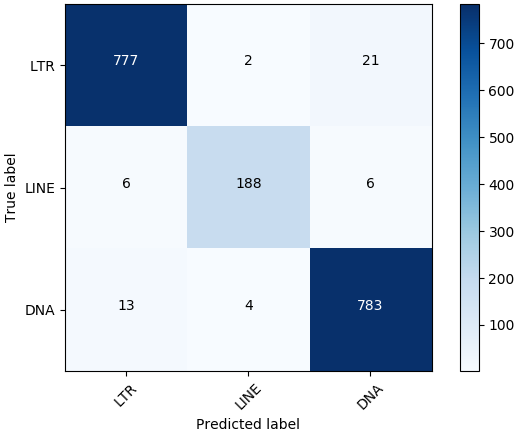
\includegraphics[width=0.7\textwidth]{./Figuras/mc-o-teste6.png}
                \caption{Matriz de confusão obtida pelo método proposto}
                \label{fig:mc-o-teste1}
            \end{figure}       
        \end{column}
        \begin{column}{0.5\textwidth}  %%<--- here
            \begin{figure}
                \centering
                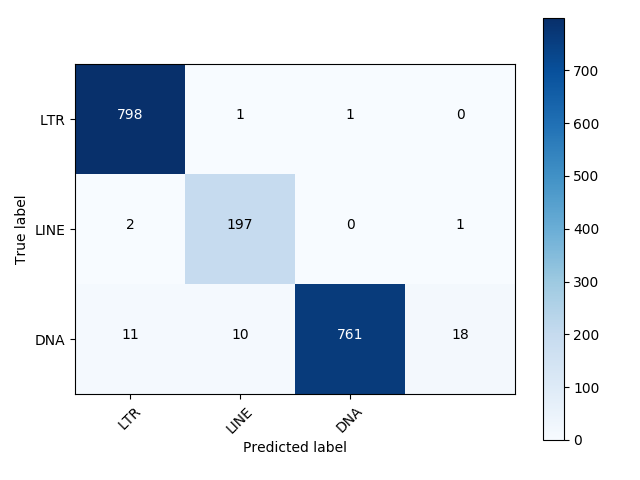
\includegraphics[width=0.8\textwidth]{./Figuras/teclass-o-ds1.png}
                \caption{Matriz de confusão obtida pelo método TEclass}
                \label{fig:mc-o-teclass-ds1}
            \end{figure}
        \end{column}
    \end{columns}
\end{frame}

\begin{frame}{\sectiontitle{sec:expres}}{Resultados - Experimento 1}
    \mode<presentation>{\vfill}
    Experimento 1 - Classificação das sequências do \textit{dataset} 1
    \begin{table}[H]
        \centering
        \caption{Dados estatísticos extraídos a partir dos resultados obtidos pelos métodos}
        \label{tab:teste1-o-results}
        \resizebox{0.7\textwidth}{!}{\begin{tabular}{|c|l|l|l|l|l|l|}
            \hline
            \rowcolor[HTML]{C0C0C0} 
            \multicolumn{1}{|l|}{\cellcolor[HTML]{C0C0C0}\textbf{Métodos}} & \textbf{Classes}        & \textbf{Acurácia}                     & \textbf{Erro}                         & \textbf{Precisão}                     & \textit{\textbf{Recall}}              & \textit{\textbf{F1-score}}            \\ \hline
            \cellcolor[HTML]{EFEFEF}                                       & \textbf{LTR}            & 0.977                                 & 0.023                                 & 0.976                                 & 0.971                                 & 0.974                                 \\ \cline{2-7} 
            \rowcolor[HTML]{EFEFEF} 
            \cellcolor[HTML]{EFEFEF}                                       & \textbf{LINE}           & {\color[HTML]{9A0000} 0.990}          & {\color[HTML]{9A0000} 0.010}          & {\color[HTML]{9A0000} 0.969}          & 0.940                                 & 0.954                                 \\ \cline{2-7} 
            \cellcolor[HTML]{EFEFEF}                                       & \textbf{DNA}            & 0.976                                 & 0.024                                 & 0.967                                 & {\color[HTML]{9A0000} 0.979}          & {\color[HTML]{9A0000} 0.973}          \\ \cline{2-7} 
            \rowcolor[HTML]{C0C0C0} 
            \cellcolor[HTML]{EFEFEF}                                       & \textbf{Média}          & {\color[HTML]{9A0000} \textbf{0.981}} & {\color[HTML]{9A0000} \textbf{0.019}} & {\color[HTML]{9A0000} \textbf{0.971}} & \textbf{0.963}                        & \textbf{0.967}                        \\ 
            \cline{2-7}
            \rowcolor[HTML]{C0C0C0}
            \cellcolor[HTML]{EFEFEF}                                       & \textbf{Tempo (treino)} & \multicolumn{5}{l|}{\textbf{15m 29.486s}}                                                                                                                                                             \\ \cline{2-7} 
            \rowcolor[HTML]{C0C0C0} 
            \multirow{-6}{*}{\cellcolor[HTML]{EFEFEF}\textbf{CNNTEclass}}  & \textbf{Tempo (teste)}  & \multicolumn{5}{l|}{\cellcolor[HTML]{C0C0C0}{\color[HTML]{9A0000} \textbf{0m 2.291s}}}                                                                                                                \\ \hline
            \cellcolor[HTML]{EFEFEF}                                       & \textbf{LTR}            & {\color[HTML]{9A0000} 0.981}          & {\color[HTML]{9A0000} 0.019}          & {\color[HTML]{9A0000} 0.984}          & {\color[HTML]{9A0000} 0.998}          & {\color[HTML]{9A0000} 0.991}          \\ \cline{2-7} 
            \rowcolor[HTML]{EFEFEF} 
            \cellcolor[HTML]{EFEFEF}                                       & \textbf{LINE}           & 0.982                                 & 0.018                                 & 0.943                                 & {\color[HTML]{9A0000} 0.985}          & {\color[HTML]{9A0000} 0.963}          \\ \cline{2-7} 
            \cellcolor[HTML]{EFEFEF}                                       & \textbf{DNA}            & {\color[HTML]{9A0000} 0.977}          & {\color[HTML]{9A0000} 0.023}          & {\color[HTML]{9A0000} 0.976}          & 0.951                                 & 0.963                                 \\ \cline{2-7} 
            \rowcolor[HTML]{C0C0C0} 
            \cellcolor[HTML]{EFEFEF}                                       & \textbf{Média}          & \textbf{0.980}                        & \textbf{0.020}                        & \textbf{0.967}                        & {\color[HTML]{9A0000} \textbf{0.978}} & {\color[HTML]{9A0000} \textbf{0.972}} \\ \cline{2-7}
            \rowcolor[HTML]{C0C0C0}
            \multirow{-5}{*}{\cellcolor[HTML]{EFEFEF}\textbf{TEclass}}     & \textbf{Tempo (teste)}  & \multicolumn{5}{l|}{\textbf{3m 32.520s}}                                                                                                                                                              \\ \hline
        \end{tabular}}
    \end{table}
\end{frame}

\begin{frame}{\sectiontitle{sec:expres}}{Resultados - Experimento 2}
    \mode<presentation>{\vfill}
    Experimento 2 - Classificação das sequências do \textit{dataset} 2 a nível de superfamília
    \begin{figure}[H]
        \centering
        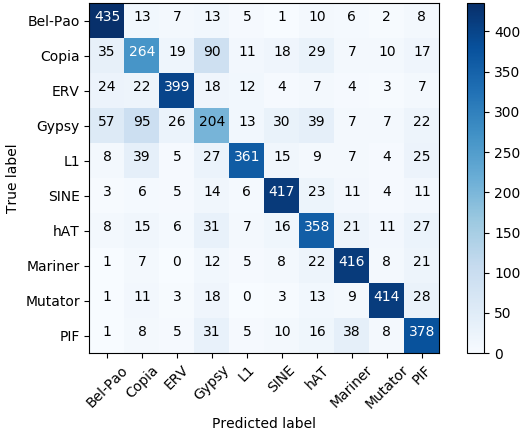
\includegraphics[width=0.4\textwidth]{./Figuras/mc-sf-teste7.png}
        \caption{Matriz de confusão obtida pelo método proposto}
        \label{fig:mc-sf-teste2}
    \end{figure}       
\end{frame}

\begin{frame}{\sectiontitle{sec:expres}}{Resultados - Experimento 2}
    \mode<presentation>{\vfill}
    Experimento 2 - Classificação das sequências do \textit{dataset} 2 a nível de superfamília
    \begin{table}[H]
        \centering
        \caption{Dados estatísticos extraídos a partir dos resultados obtidos pela classificação a nível de superfamília}
        \label{tab:teste7-sf-results}
        \resizebox{0.5\textwidth}{!}{\begin{tabular}{|l|l|l|l|l|l|}
            \hline
            \rowcolor[HTML]{C0C0C0} 
            \textbf{Classe}  & \textbf{Acurácia} & \textbf{Erro}  & \textbf{Precisão} & \textit{\textbf{Recall}} & \textit{\textbf{F1-score}} \\ \hline
            \textbf{Bel-Pao} & 0.959             & 0.041          & 0.759             & 0.870                    & 0.811                      \\ \hline
            \rowcolor[HTML]{EFEFEF} 
            \textbf{Copia}   & 0.910             & 0.090          & 0.550             & 0.528                    & 0.539                      \\ \hline
            \textbf{ERV}     & 0.965             & 0.035          & 0.840             & 0.798                    & 0.818                      \\ \hline
            \rowcolor[HTML]{EFEFEF} 
            \textbf{Gypsy}   & 0.890             & 0.110          & 0.445             & 0.408                    & 0.426                      \\ \hline
            \textbf{L1}      & 0.959             & 0.041          & 0.849             & 0.722                    & 0.781                      \\ \hline
            \rowcolor[HTML]{EFEFEF} 
            \textbf{SINE}    & 0.962             & 0.038          & 0.799             & 0.834                    & 0.816                      \\ \hline
            \textbf{hAT}     & 0.938             & 0.062          & 0.681             & 0.716                    & 0.698                      \\ \hline
            \rowcolor[HTML]{EFEFEF} 
            \textbf{Mariner} & 0.961             & 0.039          & 0.791             & 0.832                    & 0.811                      \\ \hline
            \textbf{Mutator} & 0.971             & 0.029          & 0.879             & 0.828                    & 0.853                      \\ \hline
            \rowcolor[HTML]{EFEFEF} 
            \textbf{PIF}     & 0.942             & 0.058          & 0.695             & 0.756                    & 0.724                      \\ \hline
            \rowcolor[HTML]{C0C0C0} 
            \textbf{Média}   & \textbf{0.946}    & \textbf{0.054} & \textbf{0.729}    & \textbf{0.729}           & \textbf{0.728}             \\ \hline
        \end{tabular}}
    \end{table}
\end{frame}

\begin{frame}{\sectiontitle{sec:expres}}{Resultados - Experimento 2}
    \mode<presentation>{\vfill}
    Experimento 2 - Classificação das sequências do \textit{dataset} 2 a nível de ordem
    \begin{columns}
        \begin{column}{0.5\textwidth}
            \begin{figure}[H]
                \centering
                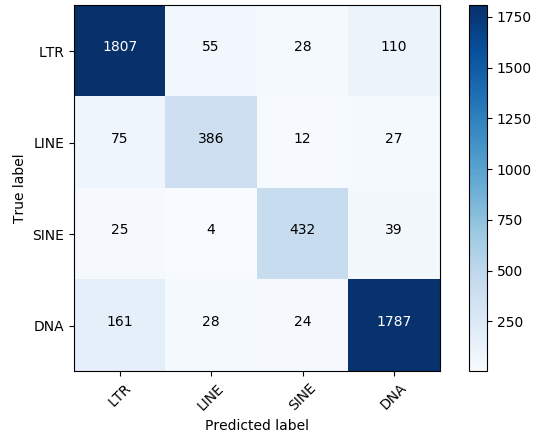
\includegraphics[width=0.7\textwidth]{./Figuras/mc-o-teste9.png}
                \caption{Matriz de confusão obtida pelo método proposto}
                \label{fig:mc-o-teste2}
            \end{figure}       
        \end{column}
        \begin{column}{0.5\textwidth}  %%<--- here
            \begin{figure}
                \centering
                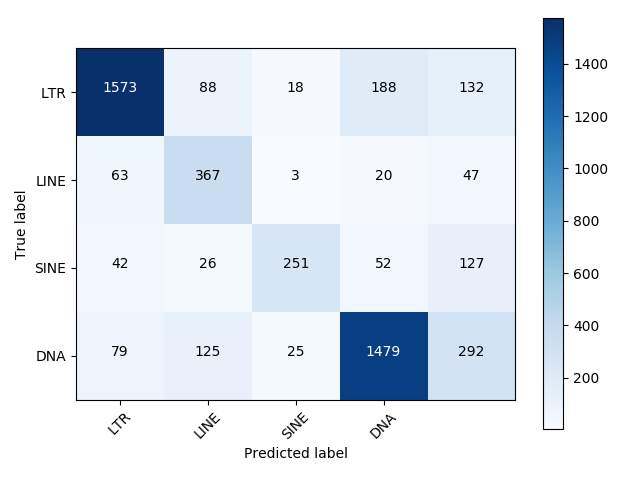
\includegraphics[width=0.8\textwidth]{./Figuras/teclass-o-ds2.png}
                \caption{Matriz de confusão obtida pelo método TEclass}
                \label{fig:mc-o-teclass-ds2}
            \end{figure}
        \end{column}
    \end{columns}
\end{frame}

\begin{frame}{\sectiontitle{sec:expres}}{Resultados - Experimento 2}
    \mode<presentation>{\vfill}
    Experimento 2 - Classificação das sequências do \textit{dataset} 2 a nível de ordem
    \begin{table}[H]
        \centering
        \caption{Dados estatísticos extraídos a partir dos resultados obtidos pelos métodos}
        \label{tab:teste2-o-results}
        \resizebox{0.7\textwidth}{!}{\begin{tabular}{|c|l|l|l|l|l|l|}
            \hline
            \rowcolor[HTML]{C0C0C0} 
            \multicolumn{1}{|l|}{\cellcolor[HTML]{C0C0C0}\textbf{Métodos}} & \textbf{Classes}                               & \textbf{Acurácia}                     & \textbf{Erro}                         & \textbf{Precisão}                     & \textit{\textbf{Recall}}              & \textit{\textbf{F1-score}}            \\ \hline
            \rowcolor[HTML]{FFFFFF} 
            \cellcolor[HTML]{EFEFEF}                                       & \textbf{LTR}                                   & {\color[HTML]{9A0000} 0.912}          & {\color[HTML]{9A0000} 0.088}          & {\color[HTML]{9A0000} 0.876}          & {\color[HTML]{9A0000} 0.909}          & {\color[HTML]{9A0000} 0.892}          \\ \cline{2-7} 
            \rowcolor[HTML]{EFEFEF} 
            \cellcolor[HTML]{EFEFEF}                                       & \textbf{LINE}                                  & {\color[HTML]{9A0000} 0.961}          & {\color[HTML]{9A0000} 0.039}          & {\color[HTML]{9A0000} 0.843}          & {\color[HTML]{9A0000} 0.752}          & {\color[HTML]{9A0000} 0.795}          \\ \cline{2-7} 
            \rowcolor[HTML]{FFFFFF} 
            \cellcolor[HTML]{EFEFEF}                                       & \textbf{SINE}                                  & {\color[HTML]{9A0000} 0.979}          & {\color[HTML]{9A0000} 0.021}          & {\color[HTML]{9A0000} 0.969}          & {\color[HTML]{9A0000} 0.814}          & {\color[HTML]{9A0000} 0.885}          \\ \cline{2-7} 
            \rowcolor[HTML]{EFEFEF} 
            \cellcolor[HTML]{EFEFEF}                                       & \textbf{DNA}                                   & {\color[HTML]{9A0000} 0.919}          & {\color[HTML]{9A0000} 0.081}          & {\color[HTML]{9A0000} 0.887}          & {\color[HTML]{9A0000} 0.913}          & {\color[HTML]{9A0000} 0.900}          \\ \cline{2-7} 
            \rowcolor[HTML]{FFFFFF} 
            \cellcolor[HTML]{EFEFEF}                                       & \textbf{Média}                                 & {\color[HTML]{9A0000} \textbf{0.943}} & {\color[HTML]{9A0000} \textbf{0.057}} & {\color[HTML]{9A0000} \textbf{0.894}} & {\color[HTML]{9A0000} \textbf{0.847}} & {\color[HTML]{9A0000} \textbf{0.868}} \\ \cline{2-7} 
            \rowcolor[HTML]{C0C0C0} 
            \cellcolor[HTML]{EFEFEF}                                       & {\color[HTML]{000000} \textbf{Tempo (treino)}} & \multicolumn{5}{l|}{\cellcolor[HTML]{C0C0C0}{\color[HTML]{000000} \textbf{57m 11.154s}}}                                                                                                              \\ \cline{2-7} 
            \rowcolor[HTML]{C0C0C0} 
            \multirow{-7}{*}{\cellcolor[HTML]{EFEFEF}\textbf{CNNTEclass}}  & \textbf{Tempo (teste)}                         & \multicolumn{5}{l|}{\cellcolor[HTML]{C0C0C0}{\color[HTML]{9A0000} \textbf{0m 7.786s}}}                                                                                                                \\ \hline
            \rowcolor[HTML]{FFFFFF} 
            \cellcolor[HTML]{EFEFEF}                                       & \textbf{LTR}                                   & {\color[HTML]{000000} 0.785}          & {\color[HTML]{000000} 0.215}          & {\color[HTML]{000000} 0.833}          & {\color[HTML]{000000} 0.787}          & {\color[HTML]{000000} 0.809}          \\ \cline{2-7} 
            \rowcolor[HTML]{EFEFEF} 
            \cellcolor[HTML]{EFEFEF}                                       & \textbf{LINE}                                  & {\color[HTML]{000000} 0.815}          & {\color[HTML]{000000} 0.185}          & {\color[HTML]{000000} 0.562}          & {\color[HTML]{000000} 0.734}          & {\color[HTML]{000000} 0.637}          \\ \cline{2-7} 
            \rowcolor[HTML]{FFFFFF} 
            \cellcolor[HTML]{EFEFEF}                                       & \textbf{SINE}                                  & {\color[HTML]{000000} 0.847}          & {\color[HTML]{000000} 0.153}          & {\color[HTML]{000000} 0.592}          & {\color[HTML]{000000} 0.504}          & {\color[HTML]{000000} 0.544}          \\ \cline{2-7} 
            \rowcolor[HTML]{EFEFEF} 
            \cellcolor[HTML]{EFEFEF}                                       & \textbf{DNA}                                   & {\color[HTML]{000000} 0.782}          & {\color[HTML]{000000} 0.218}          & {\color[HTML]{000000} 0.728}          & {\color[HTML]{000000} 0.740}          & {\color[HTML]{000000} 0.734}          \\ \cline{2-7} 
            \rowcolor[HTML]{FFFFFF} 
            \cellcolor[HTML]{EFEFEF}                                       & {\color[HTML]{343434} \textbf{Média}}          & {\color[HTML]{000000} \textbf{0.807}} & {\color[HTML]{000000} \textbf{0.193}} & {\color[HTML]{000000} \textbf{0.679}} & {\color[HTML]{000000} \textbf{0.691}} & {\color[HTML]{000000} \textbf{0.681}} \\ \cline{2-7} 
            \rowcolor[HTML]{C0C0C0} 
            \multirow{-6}{*}{\cellcolor[HTML]{EFEFEF}\textbf{TEclass}}     & {\color[HTML]{343434} \textbf{Tempo (teste)}}  & \multicolumn{5}{l|}{\cellcolor[HTML]{C0C0C0}{\color[HTML]{343434} \textbf{9m 50.654s}}}                                                                                                               \\ \hline
        \end{tabular}}
    \end{table}
\end{frame}

\begin{frame}{\sectiontitle{sec:expres}}{Resultados - Experimento 3}
    \mode<presentation>{\vfill}
    Experimento 3 - Classificação das sequências do \textit{dataset} 3
    \begin{columns}
        \begin{column}{0.5\textwidth}
            \begin{figure}[H]
                \centering
                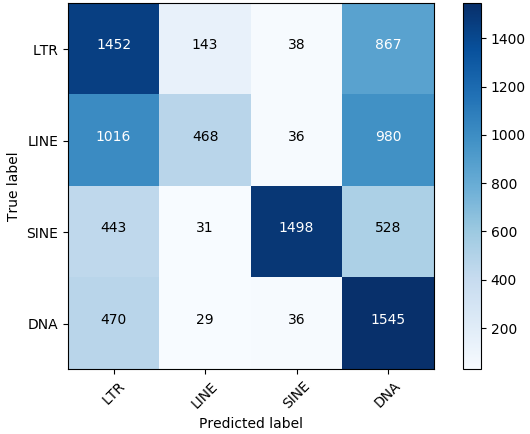
\includegraphics[width=0.7\textwidth]{./Figuras/mc-o-teste11.png}
                \caption{Matriz de confusão obtida pelo método proposto}
                \label{fig:mc-o-teste3}
            \end{figure}       
        \end{column}
        \begin{column}{0.5\textwidth}  %%<--- here
            \begin{figure}
                \centering
                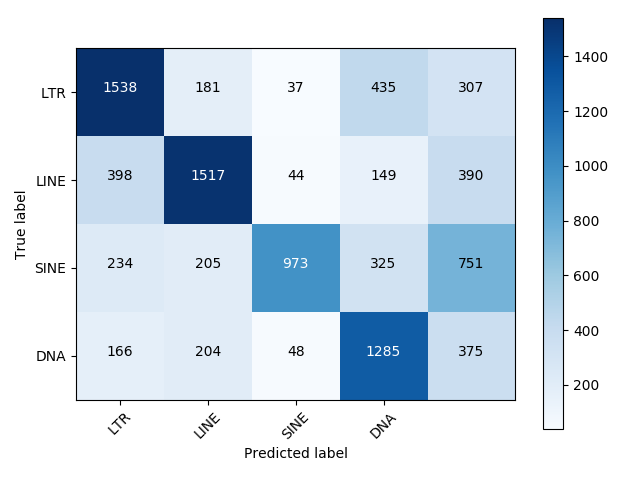
\includegraphics[width=0.8\textwidth]{./Figuras/teclass-o-ds3.png}
                \caption{Matriz de confusão obtida pelo método TEclass}
                \label{fig:mc-o-teclass-ds3}
            \end{figure}
        \end{column}
    \end{columns}
\end{frame}

\begin{frame}{\sectiontitle{sec:expres}}{Resultados - Experimento 3}
    \mode<presentation>{\vfill}
    Experimento 3 - Classificação das sequências do \textit{dataset} 3
    \begin{table}[H]
        \centering
        \caption{Dados estatísticos extraídos a partir dos resultados obtidos pelos métodos}
        \label{tab:teste3-o-results}
        \resizebox{0.7\textwidth}{!}{\begin{tabular}{|c|l|l|l|l|l|l|}
            \hline
            \rowcolor[HTML]{C0C0C0} 
            \multicolumn{1}{|l|}{\cellcolor[HTML]{C0C0C0}\textbf{Métodos}} & \textbf{Classes}                               & \textbf{Acurácia}                     & \textbf{Erro}                         & \textbf{Precisão}                     & \textit{\textbf{Recall}}              & \textit{\textbf{F1-score}}            \\ \hline
            \rowcolor[HTML]{FFFFFF} 
            \cellcolor[HTML]{EFEFEF}                                       & \textbf{LTR}                                   & {\color[HTML]{9A0000} 0.701}          & {\color[HTML]{9A0000} 0.299}          & {\color[HTML]{000000} 0.434}          & {\color[HTML]{000000} 0.483}          & {\color[HTML]{000000} 0.457}          \\ \cline{2-7} 
            \rowcolor[HTML]{EFEFEF} 
            \cellcolor[HTML]{EFEFEF}                                       & \textbf{LINE}                                  & {\color[HTML]{9A0000} 0.760}          & {\color[HTML]{9A0000} 0.240}          & {\color[HTML]{9A0000} 0.625}          & {\color[HTML]{000000} 0.205}          & {\color[HTML]{000000} 0.309}          \\ \cline{2-7} 
            \rowcolor[HTML]{FFFFFF} 
            \cellcolor[HTML]{EFEFEF}                                       & \textbf{SINE}                                  & {\color[HTML]{9A0000} 0.885}          & {\color[HTML]{9A0000} 0.115}          & {\color[HTML]{9A0000} 0.891}          & {\color[HTML]{9A0000} 0.638}          & {\color[HTML]{9A0000} 0.744}          \\ \cline{2-7} 
            \rowcolor[HTML]{EFEFEF} 
            \cellcolor[HTML]{EFEFEF}                                       & \textbf{DNA}                                   & {\color[HTML]{9A0000} 0.703}          & {\color[HTML]{9A0000} 0.297}          & {\color[HTML]{000000} 0.408}          & {\color[HTML]{9A0000} 0.822}          & {\color[HTML]{9A0000} 0.546}          \\ \cline{2-7} 
            \rowcolor[HTML]{FFFFFF} 
            \cellcolor[HTML]{EFEFEF}                                       & \textbf{Média}                                 & {\color[HTML]{9A0000} \textbf{0.762}} & {\color[HTML]{9A0000} \textbf{0.238}} & {\color[HTML]{9A0000} \textbf{0.589}} & {\color[HTML]{000000} \textbf{0.537}} & {\color[HTML]{000000} \textbf{0.514}} \\ \cline{2-7} 
            \rowcolor[HTML]{C0C0C0} 
            \cellcolor[HTML]{EFEFEF}                                       & {\color[HTML]{000000} \textbf{Tempo (treino)}} & \multicolumn{5}{l|}{\cellcolor[HTML]{C0C0C0}{\color[HTML]{000000} \textbf{59m 17.528s}}}                                                                                                              \\ \cline{2-7} 
            \rowcolor[HTML]{C0C0C0} 
            \multirow{-7}{*}{\cellcolor[HTML]{EFEFEF}\textbf{CNNTEclass}}  & \textbf{Tempo (teste)}                         & \multicolumn{5}{l|}{\cellcolor[HTML]{C0C0C0}{\color[HTML]{9A0000} \textbf{0m 19.495s}}}                                                                                                               \\ \hline
            \rowcolor[HTML]{FFFFFF} 
            \cellcolor[HTML]{EFEFEF}                                       & \textbf{LTR}                                   & {\color[HTML]{000000} 0.658}          & {\color[HTML]{000000} 0.342}          & {\color[HTML]{9A0000} 0.582}          & {\color[HTML]{9A0000} 0.616}          & {\color[HTML]{9A0000} 0.598}          \\ \cline{2-7} 
            \rowcolor[HTML]{EFEFEF} 
            \cellcolor[HTML]{EFEFEF}                                       & \textbf{LINE}                                  & {\color[HTML]{000000} 0.686}          & {\color[HTML]{000000} 0.314}          & {\color[HTML]{000000} 0.608}          & {\color[HTML]{9A0000} 0.607}          & {\color[HTML]{9A0000} 0.607}          \\ \cline{2-7} 
            \rowcolor[HTML]{FFFFFF} 
            \cellcolor[HTML]{EFEFEF}                                       & \textbf{SINE}                                  & {\color[HTML]{000000} 0.716}          & {\color[HTML]{000000} 0.284}          & {\color[HTML]{000000} 0.525}          & {\color[HTML]{000000} 0.391}          & {\color[HTML]{000000} 0.448}          \\ \cline{2-7} 
            \rowcolor[HTML]{EFEFEF} 
            \cellcolor[HTML]{EFEFEF}                                       & \textbf{DNA}                                   & {\color[HTML]{000000} 0.671}          & {\color[HTML]{000000} 0.329}          & {\color[HTML]{9A0000} 0.500}          & {\color[HTML]{000000} 0.618}          & {\color[HTML]{000000} 0.553}          \\ \cline{2-7} 
            \rowcolor[HTML]{FFFFFF} 
            \cellcolor[HTML]{EFEFEF}                                       & {\color[HTML]{343434} \textbf{Média}}          & {\color[HTML]{000000} \textbf{0.682}} & {\color[HTML]{000000} \textbf{0.318}} & {\color[HTML]{000000} \textbf{0.554}} & {\color[HTML]{9A0000} \textbf{0.558}} & {\color[HTML]{9A0000} \textbf{0.552}} \\ \cline{2-7} 
            \rowcolor[HTML]{C0C0C0} 
            \multirow{-6}{*}{\cellcolor[HTML]{EFEFEF}\textbf{TEclass}}     & {\color[HTML]{343434} \textbf{Tempo (teste)}}  & \multicolumn{5}{l|}{\cellcolor[HTML]{C0C0C0}{\color[HTML]{343434} \textbf{19m 16.675s}}}                                                                                                              \\ \hline
        \end{tabular}}
    \end{table}
\end{frame}

% -------------------------- CONCLUSÕES ---------------------------%
\section{Conclusões}\label{sec:concl}

\begin{frame}{\sectiontitle{sec:concl}}{Conclusões}
    \mode<presentation>{\vfill}
    \begin{block}{Conclusões}
        \begin{itemize}
            \item CNNs são capazes de classificar sequências de TEs utilizando os pré-processamentos propostos
            \item CNNs são capazes de classificar sequências de TEs a nível de superfamília
            \item Classificação sem aplicação de busca por similaridade
            \item Extração de características e \textit{representation learning}
            \item Tempo de treinamento e teste
        \end{itemize}
    \end{block}
\end{frame}

\begin{frame}{\sectiontitle{sec:concl}}{Conclusões - Resultados Esperados}
    \mode<presentation>{\vfill}
    \begin{block}{Resultados esperados}
        \begin{itemize}
            \item Classificação a nível de superfamílias, várias ordens e diferentes classes
            \item Descrição de sequências sem a utilização de características definidas manualmente e/ou empiricamente (handcrafted)
            \item Resultados mais eficazes que os obtidos pelos métodos estado-da-arte
            \item Diminuição do tempo computacional para a classificação de TEs
        \end{itemize}
    \end{block}
\end{frame}

\begin{frame}{\sectiontitle{sec:concl}}{Conclusões - Cronograma}
    \mode<presentation>{\vfill}
    \begin{columns}
        \begin{column}{0.5\textwidth}
            \begin{enumerate}
                \item Defesa do projeto de mestrado (qualificação)
                \item Aplicação das sugestões da banca
                \item Realização de experimentos e análises, bem como publicação da abordagem proposta e resultados obtidos
                \item Escrita da versão final
                \item Preparação da apresentação final
                \item Defesa final do mestrado
                \item Levantamento bibliográfico
            \end{enumerate}
        \end{column}
        \begin{column}{0.5\textwidth}
            \begin{table}[H]
                \centering
                \caption{Cronograma de atividades até a conclusão do projeto de pesquisa de mestrado}
                \label{tab:cronograma}
                \resizebox{\textwidth}{!}{\begin{tabular}{|c|c|c|c|c|c|c|c|c|c|}
                    \hline
                    \multicolumn{1}{|l|}{\textbf{Atividades}} & \textbf{6/19} & \textbf{7/19} & \textbf{8/19} & \textbf{9/19} & \textbf{10/19} & \textbf{11/19} & \textbf{12/19} & \textbf{1/20} & \textbf{2/20} \\ \hline
                    \textbf{1}                                & X             & X             &               &               &                &                &                &               &               \\ \hline
                    \textbf{2}                                &               & X             & X             & X             & X              & X              & X              &               &               \\ \hline
                    \textbf{3}                                &               & X             & X             & X             & X              & X              & X              &               &               \\ \hline
                    \textbf{4}                                &               &               &               &               &                &                & X              & X             & X             \\ \hline
                    \textbf{5}                                &               &               &               &               &                &                & X              & X             & X             \\ \hline
                    \textbf{6}                                &               &               &               &               &                &                &                &               & X             \\ \hline
                    \textbf{7}                                & X             & X             & X             & X             & X              & X              & X              & X             & X             \\ \hline
                \end{tabular}}
            \end{table}
        \end{column}
    \end{columns}
\end{frame}

\begin{frame}{\sectiontitle{sec:concl}}{Conclusões - Publicações Geradas}
    \mode<presentation>{\vfill}
    \begin{itemize}
        \item Cruz, M. H.P., Saito, P. T. M., Paschoal, A. R. e Bugatti, P. H. Classification of Transposable Elements by Convolutional Neural Networks. In: Proceedings of the International Conference on Artificial Intelligence and Soft Computing, pp. 1--12, Lecture Notes in Computer Science - Elsevier, 2019. (Qualis A2)
    \end{itemize}
\end{frame}

\mode<presentation>{%% Modo apresentação --- Referências
  \section{Referências}\label{sec:ref}%
  \begin{frame}[allowframebreaks]{\sectiontitle{sec:ref}}{~}%
  \printbibliography[heading = none]%
  \end{frame}%
}

\mode<article>{\printbibliography}%% Modo artigo --- Referências

\section*{Agradecimentos}\label{sec:agrad}

\begin{frame}[c]{\sectiontitle{sec:agrad}}{\mode<presentation>{~}}
Pelo apoio recebido para o desenvolvimento deste trabalho:
\mode<presentation>{\vfill}%% Modo apresentação --- Espaçamento vertical
\begin{center}

\includegraphics[height = \logoheight]{./Logos/logo-capes}
\hfill

\includegraphics[height = \logoheight]{./Logos/logo-cnpq}
\hfill

\includegraphics[height = \logoheight]{./Logos/logo-fa}
\mode<presentation>{\vfill}%% Modo apresentação --- Espaçamento vertical

\includegraphics[height = \logoheight]{./Logos/logo-utfpr}
\end{center}
\end{frame}

\mode<presentation>{%% Modo apresentação --- Agradecimentos
  \begin{frame}[c]{\sectiontitle{sec:agrad}}{~}%
    \vfill%
    \begin{center}%
      \begin{Huge}%
        Por sua atenção!%
      \end{Huge}%
    \end{center}%
    \vfill%
  \end{frame}%
}

%% Fim do documento
\end{document}
